\section{Experimental Difficulties}
\label{sec:nltr-expr-diff}

\subsection{Ferromagnetic Nanorods as a Nonlinear Beacon}

In order to generate a harmonic response, the nonlinear object must possess inherent nonlinearity in its material properties. Since TR uses electromagnetic waves, we are interested in possible nonlinear electric or magnetic properties. In this section, we discuss a potential magnetic nonlinear object in the form of ferromagnetic nanorods. These nanorods have a nonlinear magnetization curve. This means that the B-field generated from an interrogation signal should have a harmonic response that we may use for NLTR. We chose to use ferromagnetic nanorods specifically due to the potential medical application of hyperthermic treatment of tumors. The NLTR process may supply sufficient power needed to raise the temperature of the tumor, destroying it. Ferromagnetic nanorods may be injected into a tumor site as a nonlinear beacon, allowing this potential life-saving procedure to become a reality.

While the usage of diodes as nonlinear objects has been well-documented, the usage of ferromagnetic nanorods as nonlinear objects has not. As a result, we performed preliminary experiments on the ferromagnetic nanorods in order to determine whether or not the nonlinear response would be strong enough to successfully complete the NLTR process.

This preliminary experiment involved attaching ferromagnetic nanorods to an antenna (as shown in Figure~\ref{fig:nltr-nanorod-coil}), sending a pulse signal through that antenna, and then recording the response. In order to record the response, we used a spectrum analyzer, as shown in Figure~\ref{fig:nltr-nanorod-setup}. By transforming the response signal to the frequency domain, we were able to easily identify whether or not a harmonic was generated.

\begin{figure}[t]
    \centering
    \begin{minipage}[b]{.4\textwidth}
        \centering
        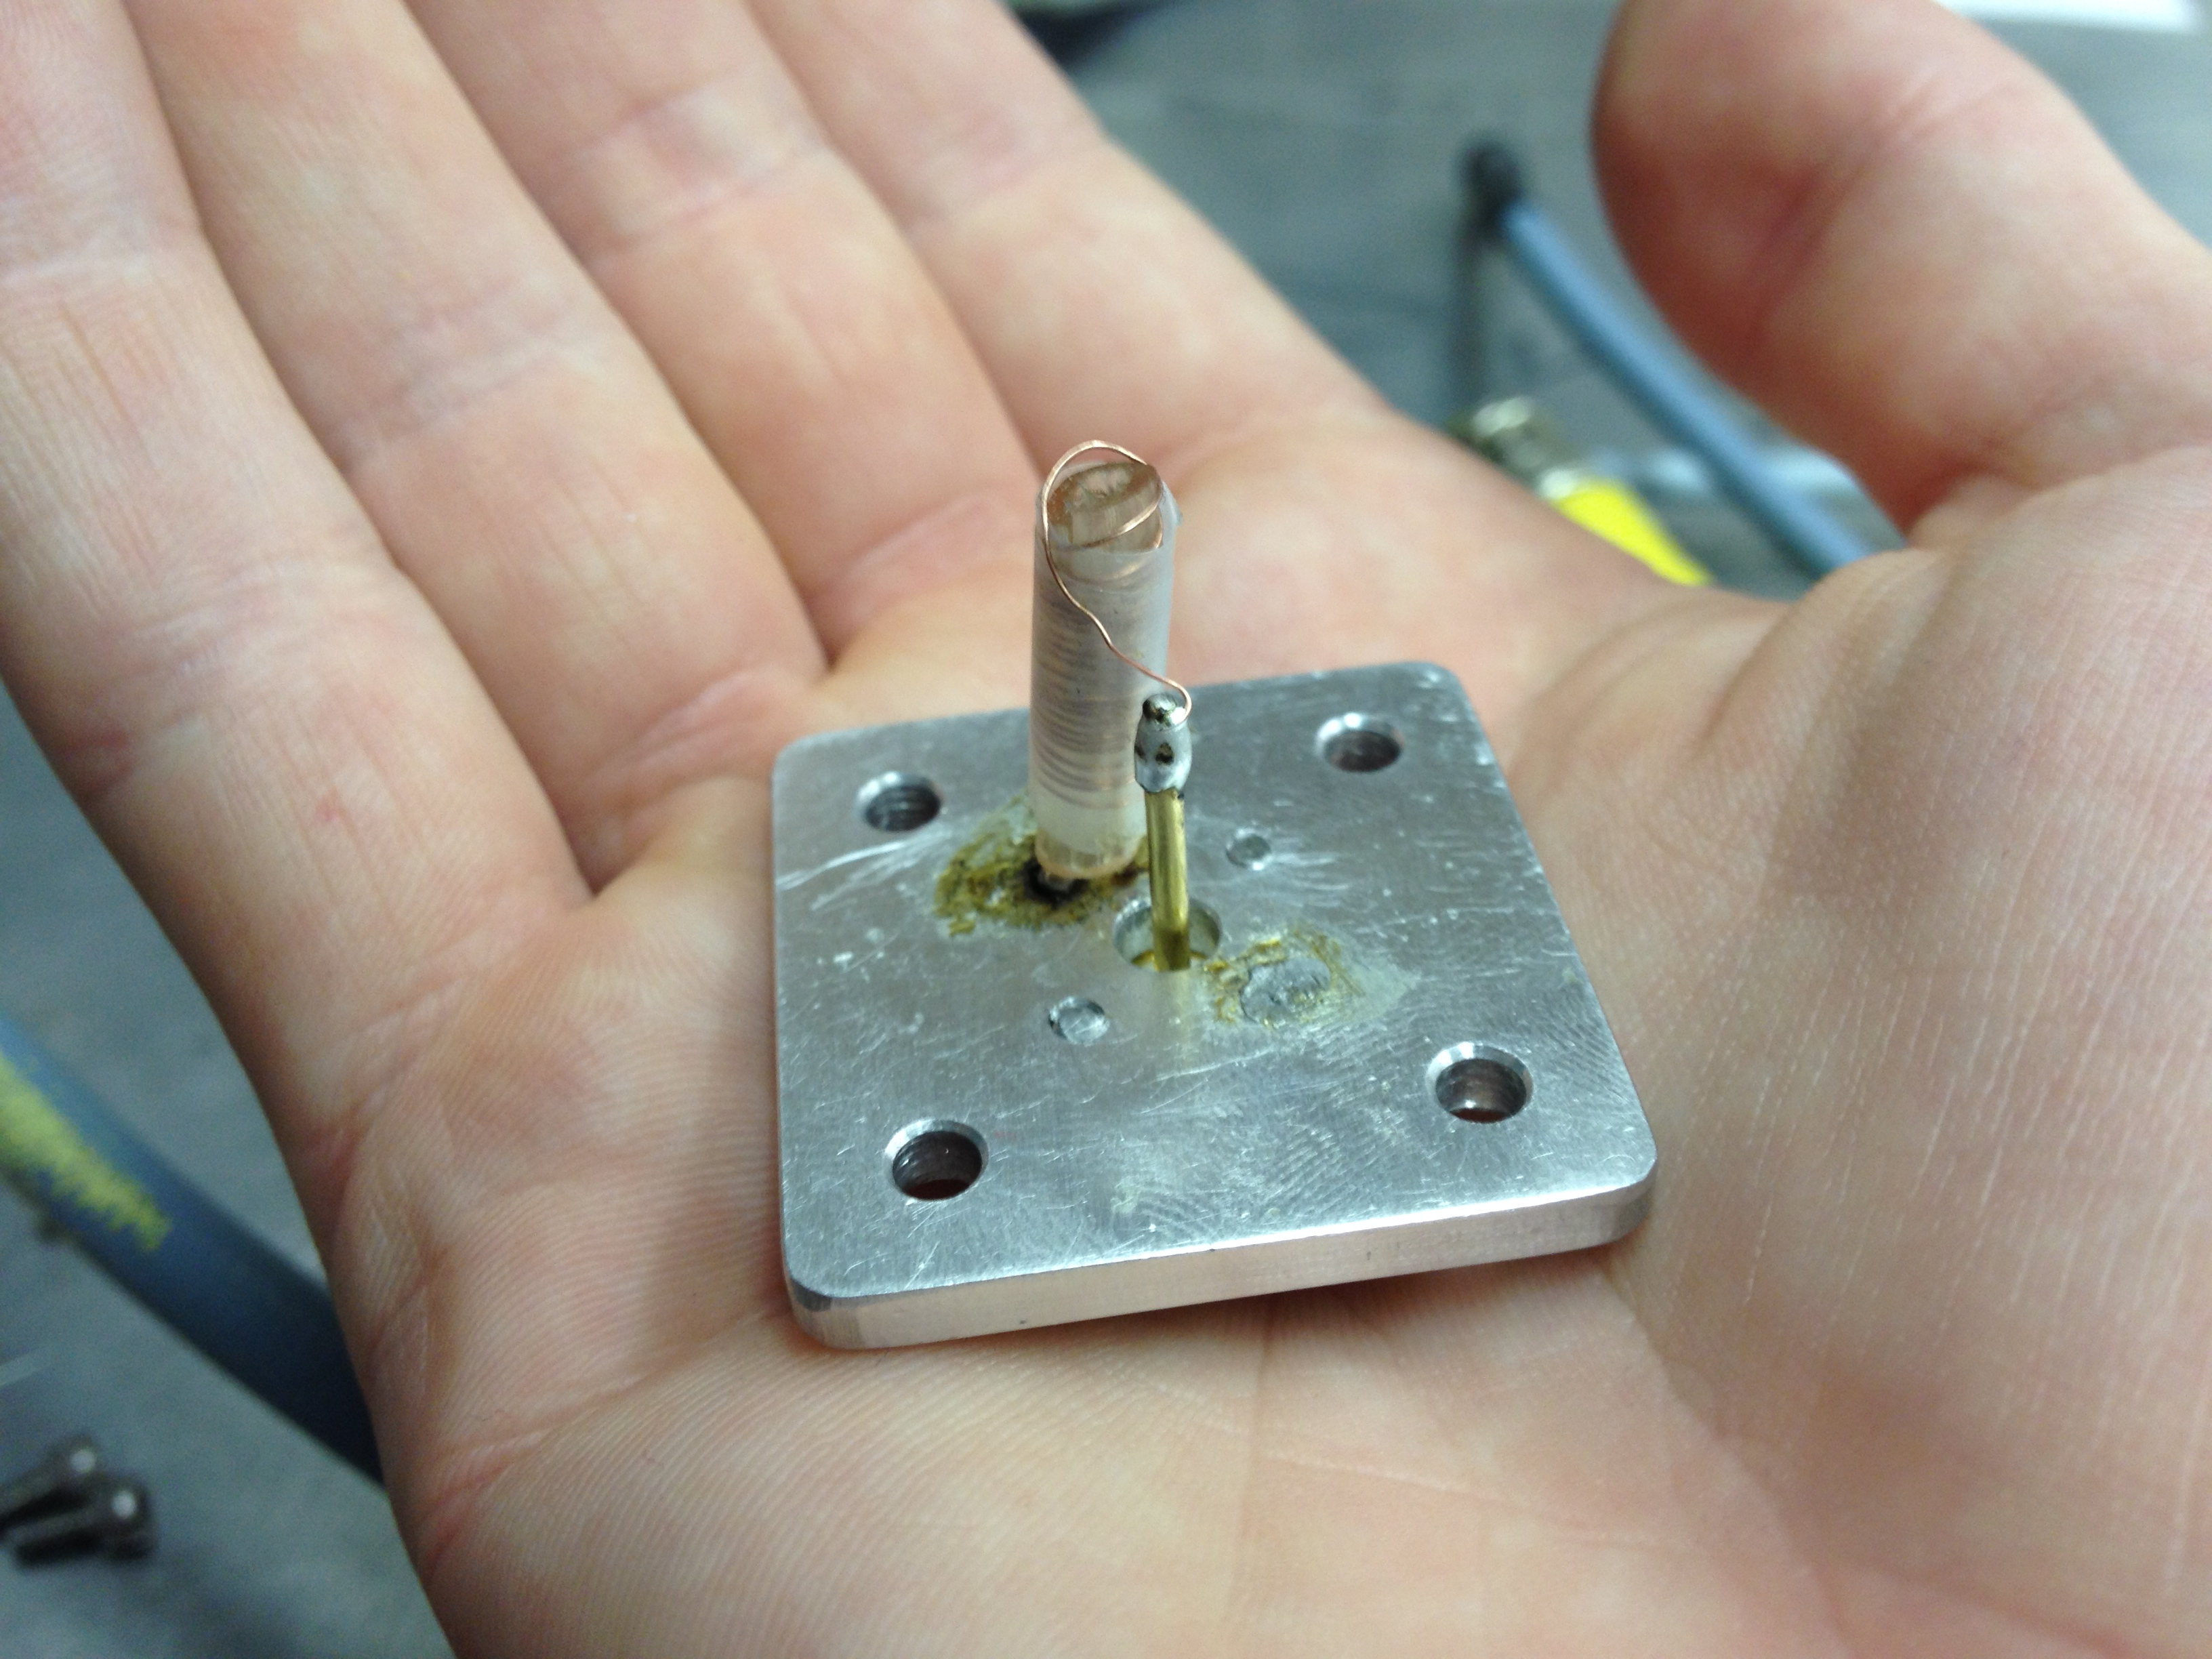
\includegraphics[width=0.9\linewidth]{nanorod/coil}
        \caption[Nanorods attached to antenna]{Antenna used for nanorod experiments. The nanorods are within the coil conntected to the monopole. The coil was used to maximize the magnetic field applied to the nanorods during use.}
        \label{fig:nltr-nanorod-coil}
    \end{minipage}
    \hfill
    \begin{minipage}[b]{.4\textwidth}
        \centering
        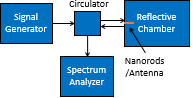
\includegraphics[width=0.9\linewidth]{nanorod/setup}
        \caption[Nanorod experimental setup]{Nanorod experimental setup. The reflective chamber and equipment used is identical to that discussed in ~\ref{fig:linear-gigabox}.}
        \label{fig:nltr-nanorod-setup}
    \end{minipage}
\end{figure}


 \begin{figure}
     \centering
     \begin{subfigure}{0.45\textwidth}
         \centering
         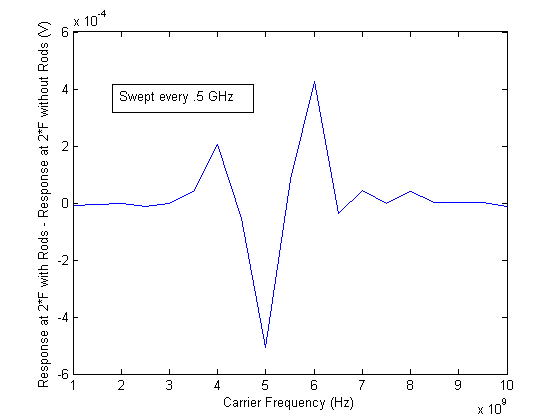
\includegraphics[width=1.0\linewidth]{nanorod/exp-1}
         \caption[]{}
         \label{fig:nanorod-exp-1}
     \end{subfigure}
         \begin{subfigure}{0.45\textwidth}
         \centering
         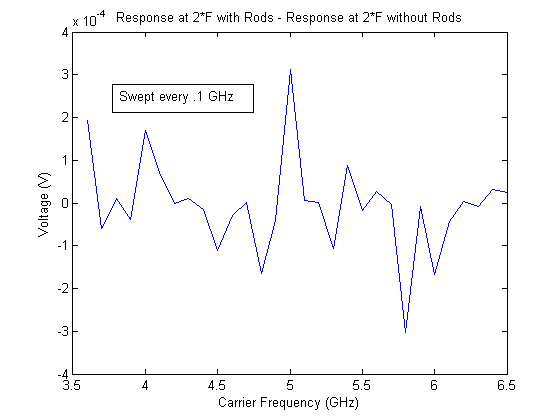
\includegraphics[width=1.0\linewidth]{nanorod/exp-2}
         \caption[]{}
         \label{fig:nanorod-exp-2}
     \end{subfigure}
         \begin{subfigure}{0.45\textwidth}
         \centering
         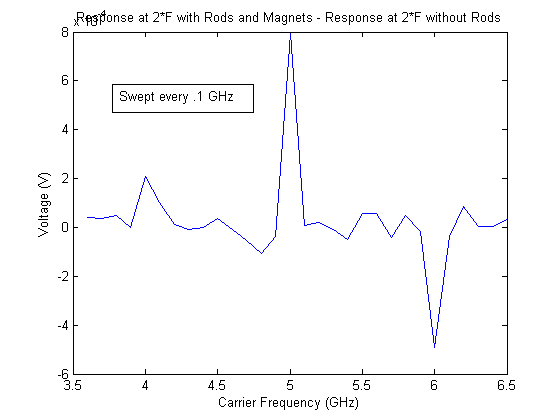
\includegraphics[width=1.0\linewidth]{nanorod/exp-3}
         \caption[]{}
         \label{fig:nanorod-exp-3}
     \end{subfigure}
         \begin{subfigure}{0.45\textwidth}
         \centering
         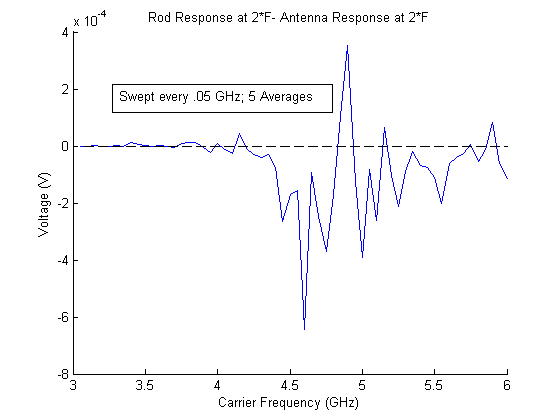
\includegraphics[width=1.0\linewidth]{nanorod/exp-4}
         \caption[]{}
         \label{fig:nanorod-exp-4}
     \end{subfigure}
     \caption[Ferromagnetic nanorod experimental results]{Experimental results. (a) - (d) show various ferromagnetic nanorod configurations' response spectra. No configuration leads to a significant $2f$ response, as illustrated through the random and small amplitude response signals}
     \label{fig:nanorod-results}
 \end{figure}

Figure~\ref{fig:nanorod-results}(a)-(d) show the $2f$ response under a variety of conditions. Although there seem to be peaks in (a) - (d), the peaks are somewhat randomly distributed and are small in magnitude.

In these experiments, we expected and searched for a $2f$ (second-order) harmonic response, because this has been observed in prior work with diodes. However, we realized later that ferromagnetic nanorods have been found to produce a noticable \textit{third-order} ($3f$) harmonic repsonse~\cite{nanorod-third-order}. As a result, we are unable to conclude from our experiments whether or not ferromagnetic nanorods would provide a sufficient nonlinear response for performing NLTR. Future work should conduct similar experiments, but focus on the $3f$ frequency range instead.

\subsection{Diodes as an Electric Nonlinear Beacon}

While utilizing a nonlinear magnetic response was not feasible, utilizing a nonlinear electric response has been well-documented through the use of a diode. This represents a nonlinear object, as the current response to an applied voltage for a diode changes significantly after a certain applied voltage value, as seen in Frazier et al. have previously used diodes in NLTR experiments to much success.

We performed another preliminary test to verify the nonlinear response of a diode after being interrogated by a Gaussian pulse. Given the history of diodes in NLTR, we believed that we would see a large $2f$ response. While performing these preliminary tests we were unable to produce any measurable harmonic from a diode while it was present in the \giga{}. In order to circumvent this problem, we used extremely large amplifiers as done by Hong et al. in their NLTR experiments. We were still unable to generate a significant harmonic response.

As a last effort we used various frequency multipliers to generate a nonlinear signal. We did this to verify that the equipment used in our setup was functioning properly. We were able to extract a nonlinear sona from the frequency multiplier; however, this is impractical for WPT as frequency multipliers are large in size. This confirmed that our equipment were working properly, but that we were unable to generate a large response. Since we were not able to generate a nonlinear sona experimentally, we conducted all of our NLTR experiments using numerical simulation.
